\documentclass[12pt,a4paper]{article}

% ─── Page Layout ───────────────────────────────────────────────────────────────
\usepackage[a4paper, margin=0.8in, headheight=14pt]{geometry}

% ─── Fonts (XeLaTeX) ───────────────────────────────────────────────────────────
\usepackage{fontspec}
\usepackage{unicode-math}
\setmainfont{TeX Gyre Pagella}
\setmonofont[Scale=0.88]{TeX Gyre Cursor}
\setmathfont{Latin Modern Math}

% ─── Packages ──────────────────────────────────────────────────────────────────
\usepackage{xcolor}
\usepackage{colortbl}
\usepackage{titlesec}
\usepackage{enumitem}
\usepackage{tabularx}
\usepackage{booktabs}
\usepackage{array}
\usepackage{amsmath}
\usepackage{tikz}
\usetikzlibrary{shapes.geometric, arrows.meta, positioning, calc, fit, decorations.pathreplacing}
\usepackage{tcolorbox}
\tcbuselibrary{skins, breakable}
\usepackage{hyperref}
\usepackage{fancyhdr}
\usepackage{graphicx}
\usepackage{microtype}
\hyphenpenalty=10000
\exhyphenpenalty=10000
\sloppy
\usepackage{caption}
\usepackage{setspace}
\usepackage{multirow}
\usepackage{tocloft}

% ─── Q&A helper ────────────────────────────────────────────────────────────────
\newcommand{\Q}[1]{\textbf{#1}\par\noindent\ignorespaces}

% ─── Colour Palette ────────────────────────────────────────────────────────────
\definecolor{myred}{RGB}{196,30,58}
\definecolor{mydark}{RGB}{30,30,50}
\definecolor{mygreen}{RGB}{14,120,80}
\definecolor{myteal}{RGB}{0,130,140}
\definecolor{myamber}{RGB}{180,100,0}
\definecolor{mypurple}{RGB}{100,30,160}
\definecolor{mygray}{RGB}{246,247,249}
\definecolor{mgframe}{RGB}{180,185,200}
\definecolor{watermark}{RGB}{145,150,170}
\definecolor{hdrred}{RGB}{250,232,235}
\definecolor{hdrgreen}{RGB}{220,244,233}
\definecolor{hdrteal}{RGB}{220,242,244}
\definecolor{hdramber}{RGB}{253,242,215}
\definecolor{hdrpurple}{RGB}{238,228,255}
\definecolor{hdrgray}{RGB}{238,240,245}
\definecolor{rowalt}{RGB}{250,251,253}

% ─── Section Formatting ────────────────────────────────────────────────────────
\titleformat{\section}
  {\large\bfseries\color{myred}}{\thesection.}{0.5em}{}
  [\vspace{1pt}{\color{myred}\rule{\linewidth}{0.8pt}}]
\titleformat{\subsection}
  {\normalsize\bfseries\color{myteal}}{\thesubsection}{0.5em}{}
\titlespacing*{\section}{0pt}{18pt}{7pt}
\titlespacing*{\subsection}{0pt}{11pt}{4pt}

% ─── Paragraph ─────────────────────────────────────────────────────────────────
\setlength{\parindent}{0pt}
\setlength{\parskip}{4pt}

% ─── TOC Styling ───────────────────────────────────────────────────────────────
\renewcommand{\cfttoctitlefont}{\large\bfseries\color{myred}}
\renewcommand{\cftaftertoctitle}{\par\noindent{\color{myred}\rule{\linewidth}{0.8pt}}}
\setlength{\cftbeforetoctitleskip}{0pt}
\setlength{\cftaftertoctitleskip}{6pt}
\renewcommand{\cftsecfont}{\normalsize\bfseries\color{mydark}}
\renewcommand{\cftsecpagefont}{\normalsize\bfseries\color{mydark}}
\renewcommand{\cftsecleader}{\cftdotfill{\cftdotsep}}
\setlength{\cftbeforesecskip}{7pt}
\renewcommand{\cftsubsecfont}{\small\color{mydark}}
\renewcommand{\cftsubsecpagefont}{\small\color{mydark}}
\setlength{\cftbeforesubsecskip}{3pt}
\setlength{\cftsubsecindent}{1.4em}

% ─── Table helpers ─────────────────────────────────────────────────────────────
\renewcommand{\arraystretch}{1.45}
\setlength{\tabcolsep}{6pt}
\arrayrulecolor{mydark}
\newcolumntype{B}[1]{>{\small\bfseries\raggedright\arraybackslash}m{#1}}
\newcolumntype{Y}{>{\small\raggedright\arraybackslash}X}
\renewcommand{\tabularxcolumn}[1]{m{#1}}

% ─── Header / Footer ───────────────────────────────────────────────────────────
\pagestyle{fancy}
\fancyhf{}
\fancyhead[L]{\small\color{myred}\textbf{PE-EC701B}\;\color{mydark}--- Satellite Communication}
\fancyhead[R]{\small\color{myteal}\textbf{Module 5 Notes}}
\fancyfoot[C]{\small\color{mydark}\thepage}
\fancyfoot[R]{\small\color{watermark}\textit{\copyright\ Biraj}}
\renewcommand{\headrulewidth}{0.5pt}
\renewcommand{\footrulewidth}{0.3pt}

% ─── Hyperref ──────────────────────────────────────────────────────────────────
\hypersetup{
  colorlinks=true, linkcolor=myteal, urlcolor=myteal,
  pdfauthor={Biraj Sarkar},
  pdftitle={PE-EC701B --- Module 5 Notes}
}

% ─── tcolorbox styles ──────────────────────────────────────────────────────────
\tcbset{
  tikzbox/.style={
    colback=mygray, colframe=mgframe, boxrule=0.6pt, arc=4pt,
    left=8pt, right=8pt, top=6pt, bottom=6pt,
    colbacktitle=mgframe, coltitle=mydark,
    fonttitle=\small\bfseries
  },
  defbox/.style={
    colback=hdrgreen, colframe=mygreen, boxrule=0.8pt, arc=4pt,
    left=9pt, right=9pt, top=6pt, bottom=6pt,
    colbacktitle=mygreen, coltitle=white,
    fonttitle=\small\bfseries
  },
  formulabox/.style={
    colback=hdrteal, colframe=myteal, boxrule=0.8pt, arc=4pt,
    left=9pt, right=9pt, top=7pt, bottom=7pt,
    colbacktitle=myteal, coltitle=white,
    fonttitle=\small\bfseries
  },
  examplebox/.style={
    colback=hdramber, colframe=myamber, boxrule=0.8pt, arc=4pt,
    left=9pt, right=9pt, top=6pt, bottom=6pt,
    colbacktitle=myamber, coltitle=white,
    fonttitle=\small\bfseries
  },
  masonbox/.style={
    colback=hdrpurple, colframe=mypurple, boxrule=0.8pt, arc=4pt,
    left=9pt, right=9pt, top=6pt, bottom=6pt,
    colbacktitle=mypurple, coltitle=white,
    fonttitle=\small\bfseries
  },
  exambox/.style={
    colback=hdrpurple, colframe=mypurple, boxrule=1pt, arc=5pt,
    left=10pt, right=10pt, top=8pt, bottom=8pt,
    colbacktitle=mypurple, coltitle=white,
    fonttitle=\bfseries,
    breakable, title after break={\textbf{Frequently Asked / Viva Questions (contd.)}}}
}
% Make all boxes breakable across pages
\tcbset{breakable}

% ─── TikZ styles ───────────────────────────────────────────────────────────────
\tikzset{
  block/.style={rectangle, draw=myteal, fill=hdrteal,
    text width=2.4cm, align=center, minimum height=0.95cm,
    font=\small, rounded corners=3pt, line width=0.7pt},
  redblock/.style={rectangle, draw=myred, fill=hdrred,
    text width=2.4cm, align=center, minimum height=0.95cm,
    font=\small, rounded corners=3pt, line width=0.7pt},
  netnode/.style={rectangle, draw=myteal, fill=hdrteal,
    text width=1.5cm, align=center, minimum height=0.8cm,
    font=\small, rounded corners=3pt, line width=0.7pt},
  sumjunc/.style={circle, draw=myamber, fill=hdramber,
    minimum size=0.62cm, font=\small, line width=0.8pt},
  snode/.style={circle, draw=mypurple, fill=hdrpurple,
    minimum size=0.55cm, font=\footnotesize, line width=0.7pt},
  arrow/.style={-Stealth, thick, color=mydark},
  redarrow/.style={-Stealth, thick, color=myred},
  line/.style={thick, color=mydark}
}

% ═══════════════════════════════════════════════════════════════════════════════
\begin{document}
% ═══════════════════════════════════════════════════════════════════════════════

\begin{center}
  {\LARGE\bfseries\color{myred} PE-EC701B --- Satellite Communication}\\[5pt]
  {\normalsize\color{mydark} Semester VII \quad$\bullet$\quad 3L:0T:0P \quad$\bullet$\quad 3 Credits}\\[3pt]
  {\normalsize\color{myteal}\textbf{Module 5 Exam Notes: Satellite Link Budget}}\\[3pt]
  {\small\color{mydark} CGEC \;$|$\; B.Tech ECE (2023--27) \;$|$\; \textit{Biraj Sarkar}}
\end{center}
\vspace{2pt}
\noindent{\color{myred}\rule{\linewidth}{1.5pt}}
\vspace{2pt}

\hypersetup{linkcolor=mydark}
\tableofcontents
\hypersetup{linkcolor=myteal}
\newpage

% ===============================================================================
\section{Power Flux Density and Received Signal Power}
% ===============================================================================

The link budget calculations track the signal power level from the ground transmitter, through the orbital space path, to the ground receiver.

\subsection{Power Flux Density (F)}
An isotropic radiator distributes its power uniformly in all directions over a sphere. At a distance $d$ from the transmitter, the power flux density ($F$) is:
\begin{equation}
  F = \frac{P_t}{4\pi d^2} \quad [\text{W/m}^2]
\end{equation}
If the transmitter uses a directional antenna with gain $G_t$, the power is concentrated, yielding:
\begin{equation}
  F = \frac{P_t G_t}{4\pi d^2} = \frac{EIRP}{4\pi d^2} \quad [\text{W/m}^2]
\end{equation}
Where $EIRP = P_t G_t$ is the \textbf{Equivalent Isotropically Radiated Power}.

\subsection{Received Signal Power ($P_r$)}
The receiving antenna intercepts a portion of this flux. The captured power is proportional to the antenna's \textbf{effective aperture area} ($A_e$):
\begin{equation}
  P_r = F \cdot A_e \quad [\text{W}]
\end{equation}
Using the fundamental antenna relation $A_e = \frac{G_r \lambda^2}{4\pi}$:
\begin{equation}
  P_r = \left( \frac{P_t G_t}{4\pi d^2} \right) \left( \frac{G_r \lambda^2}{4\pi} \right) = P_t G_t G_r \left( \frac{\lambda}{4\pi d} \right)^2 \quad [\text{W}]
\end{equation}
This is the \textbf{Friis Transmission Equation}. It can be written as:
\begin{equation}
  P_r = \frac{EIRP \cdot G_r}{L_{FSL}}
\end{equation}
Where $L_{FSL}$ is the \textbf{Free Space Path Loss (FSL)}:
\begin{equation}
  L_{FSL} = \left( \frac{4\pi d}{\lambda} \right)^2 = \left( \frac{4\pi f d}{c} \right)^2
\end{equation}
In decibels:
\begin{equation}
  L_{FSL\_dB} = 32.44 + 20\log_{10}(d_{\text{km}}) + 20\log_{10}(f_{\text{MHz}})
\end{equation}

% ===============================================================================
\section{System Noise Temperature and Noise Power}
% ===============================================================================

The performance of a receiving system is limited by thermal noise, which is modeled using an equivalent noise temperature.

\subsection{Noise Power Calculation}
The thermal noise power ($N$) generated in a receiver of bandwidth $B$ is given by:
\begin{equation}
  N = k \cdot T_s \cdot B \quad [\text{W}]
\end{equation}
Where:
\begin{itemize}[leftmargin=*, itemsep=3pt]
  \item $k = 1.38 \times 10^{-23} \text{ J/K}$ (Boltzmann's constant)
  \item $T_s$ = System Noise Temperature (Kelvin, K)
  \item $B$ = Noise Bandwidth (Hz)
\end{itemize}
In dBW:
\begin{equation}
  N_{\text{dBW}} = -228.6 + 10\log_{10}(T_s) + 10\log_{10}(B)
\end{equation}

\subsection{Calculation of System Noise Temperature ($T_s$)}
If an antenna with noise temperature $T_{ant}$ is connected to a receiver via a lossy waveguide line with loss factor $L$ ($L \ge 1$, where $L = 10^{\text{Loss\_dB}/10}$) at physical temperature $T_0 \approx 290\text{ K}$, the system noise temperature ($T_s$) referred to the receiver input is:
\begin{equation}
  T_s = \frac{T_{ant}}{L} + T_{0}\left(1 - \frac{1}{L}\right) + T_{rx}
\end{equation}
Where $T_{rx}$ is the effective noise temperature of the receiver itself, related to its noise figure $F_{rx}$ by:
\begin{equation}
  T_{rx} = T_0 (F_{rx} - 1)
\end{equation}

For a cascaded chain of amplifiers (e.g., LNA followed by mixer and down-converter), the overall receiver noise temperature is given by \textbf{Friis Formula}:
\begin{equation}
  T_{rx} = T_1 + \frac{T_2}{G_1} + \frac{T_3}{G_1 G_2} + \dots
\end{equation}
Where $T_n$ and $G_n$ are the equivalent noise temperature and linear gain of the $n$-th stage. This formula proves why a high-gain, low-noise LNA must be the first stage.

% ===============================================================================
\section{Drafting the Satellite Link Budget}
% ===============================================================================

The link budget is a tabular summation of all gains and losses along the communication path to calculate the final \textbf{Carrier-to-Noise Ratio ($C/N$)} at the receiver demodulator.

\begin{tcolorbox}[tikzbox, title={Link Budget System Model}]
\centering
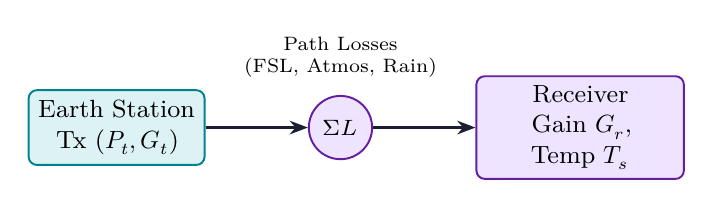
\begin{tikzpicture}[scale=0.9, every node/.style={font=\scriptsize}]
  % Ground Station
  \node[block, text width=2.0cm] (tx) {Earth Station\\Tx ($P_t, G_t$)};
  
  % Path
  \node[snode, right=1.3cm of tx] (loss) {$\Sigma L$};
  \node[above=0.1cm of loss, align=center] {Path Losses\\(FSL, Atmos, Rain)};
  
  % Satellite Receiver
  \node[block, right=1.3cm of loss, draw=mypurple, fill=hdrpurple] (sat) {Receiver\\Gain $G_r$, Temp $T_s$};
  
  % Connections
  \draw[arrow] (tx) -- (loss);
  \draw[arrow] (loss) -- (sat);
\end{tikzpicture}
\end{tcolorbox}

\subsection{Carrier-to-Noise Ratio (C/N) Expression}
The received carrier power is $C = P_r$. The carrier-to-noise ratio is:
\begin{equation}
  \frac{C}{N} = \frac{P_r}{k T_s B} = \frac{EIRP \cdot G_r}{L_{\text{losses}} \cdot k T_s B} = \left(\frac{EIRP}{L_{\text{losses}} \cdot k \cdot B}\right) \left(\frac{G_r}{T_s}\right)
\end{equation}
Where $G/T = G_r/T_s$ is the receiving system's \textbf{Figure of Merit} (expressed in $\text{dB/K}$).

In logarithmic decibel form:
\begin{equation}
  \left[\frac{C}{N}\right]_{\text{dB}} = EIRP_{\text{dBW}} - L_{\text{losses\_dB}} + \left[\frac{G}{T}\right]_{\text{dB/K}} - k_{\text{dBW}} - B_{\text{dB-Hz}}
\end{equation}
Where:
\begin{itemize}[leftmargin=*, itemsep=3pt]
  \item $k_{\text{dBW}} = -228.6 \text{ dBW/(K}\cdot\text{Hz)}$
  \item $B_{\text{dB-Hz}} = 10\log_{10}(B_{\text{Hz}})$
  \item $L_{\text{losses\_dB}} = L_{FSL} + L_{\text{atmospheric}} + L_{\text{polarization}} + L_{\text{antenna-pointing}}$
\end{itemize}

\subsection{Carrier-to-Noise Density Ratio ($C/N_0$)}
To evaluate system performance independent of receiver bandwidth, we use $C/N_0$:
\begin{equation}
  \frac{C}{N_0} = \frac{C}{N} \cdot B \quad [\text{Hz}]
\end{equation}
\begin{equation}
  \left[\frac{C}{N_0}\right]_{\text{dB-Hz}} = EIRP_{\text{dBW}} - L_{\text{losses\_dB}} + \left[\frac{G}{T}\right]_{\text{dB/K}} + 228.6
\end{equation}

% ===============================================================================
\section{Link Performance: Clear Air vs. Rainy Conditions}
% ===============================================================================

Atmospheric phenomena significantly degrade link performance, especially at frequencies above 10 GHz (Ku and Ka bands).

\subsection{Clear Air Conditions}
Under clear skies, the link is subject only to \textbf{gaseous absorption} from water vapor and oxygen molecules in the atmosphere. The attenuation is low (typically $< 0.5$ dB for C-band).

\subsection{Rainy Conditions}
Rain introduces a dual penalty on the link:
\begin{enumerate}[label=\textbf{\arabic*.}, leftmargin=*, itemsep=3pt]
  \item \textbf{Signal Attenuation ($A_{\text{rain}}$):} Rain droplets scatter and absorb the microwave energy, reducing the received carrier power ($C$) by $A_{\text{rain}}$ dB.
  \item \textbf{Increase in Noise Temperature ($\Delta T_{\text{ant}}$):} The absorbing rain medium acts as a thermal radiator, increasing the antenna noise temperature:
    \begin{equation}
      T_{ant\_rain} = T_{ant\_clear} \cdot 10^{-A_{\text{rain}}/10} + T_m \left( 1 - 10^{-A_{\text{rain}}/10} \right)
    \end{equation}
    Where $T_m$ is the physical temperature of the rain medium (typically assumed to be $275\text{ K}$ or $290\text{ K}$).
\end{enumerate}

This increase in $T_{ant}$ directly raises the system noise temperature $T_s$, thereby raising the noise floor ($N$). This combined effect severely degrades the overall received $[C/N]$ ratio.

% ===============================================================================
% MANDATORY QUICK REVISION PAGE
% ===============================================================================
\newpage
\begin{center}
  {\large\bfseries\color{myred} Quick Revision --- Module V}\\[3pt]
  {\small\color{mydark} Satellite Link Budget $|$ PE-EC701B}
\end{center}
\noindent{\color{myred}\rule{\linewidth}{1.2pt}}
\vspace{4pt}

\begin{tcolorbox}[formulabox, title={\textbf{Key Formulas at a Glance}}]
\renewcommand{\arraystretch}{1.9}
\begin{tabularx}{\linewidth}{B{5.0cm} X}
Equivalent Radiated Power & $EIRP = P_t G_t \implies EIRP_{\text{dBW}} = P_{t\text{\,dBW}} + G_{t\text{\,dBi}}$ \\[4pt]
Free Space Path Loss & $\displaystyle L_{FSL} = \left(\frac{4\pi d}{\lambda}\right)^2 \implies L_{FSL\_dB} \approx 32.44 + 20\log(d_{\text{km}}) + 20\log(f_{\text{MHz}})$ \\[4pt]
Noise Power & $N = k T_s B \implies N_{\text{dBW}} = -228.6 + 10\log(T_s) + 10\log(B)$ \\[4pt]
Friis Cascade Temperature & $\displaystyle T_{rx} = T_1 + \frac{T_2}{G_1} + \frac{T_3}{G_1 G_2} + \dots$ \\[4pt]
Carrier-to-Noise Ratio & $\displaystyle \left[\frac{C}{N}\right]_{\text{dB}} = EIRP_{\text{dBW}} - L_{\text{losses\_dB}} + \left[\frac{G}{T}\right]_{\text{dB/K}} - 10\log(B) + 228.6$
\end{tabularx}
\end{tcolorbox}

\begin{tcolorbox}[defbox, title={\textbf{One-Line Definitions}}]
\begin{itemize}[leftmargin=*, itemsep=2.5pt, topsep=0pt]
  \item \textbf{EIRP:} Equivalent power that would need to be radiated by an isotropic antenna to achieve the same directional signal strength.
  \item \textbf{Free Space Loss:} Geometrical spreading loss of electromagnetic energy as it radiates outward through space.
  \item \textbf{G/T Ratio:} Figure of merit of a receiving system, representing the ratio of antenna gain to system noise temperature.
  \item \textbf{Friis Formula:} Expression calculating the total noise temperature of cascaded receiver stages.
  \item \textbf{Boltzmann's Constant (k):} Proportionality constant relating kinetic energy to temperature ($1.38 \times 10^{-23} \text{ J/K}$).
  \item \textbf{Rain Fade Penalty:} Combined loss of carrier power and rise in receiver noise floor caused by rain.
\end{itemize}
\end{tcolorbox}

\begin{tcolorbox}[exambox, title={\textbf{Frequently Asked / Viva Questions}}]
\begin{enumerate}[topsep=0pt, label=\textbf{Q\arabic*.}, itemsep=5pt]
  \item \Q{Define EIRP and write its equation in logarithmic form.}
    Equivalent Isotropically Radiated Power. It measures the total directional power radiated. $EIRP_{\text{dBW}} = P_{t\text{\,dBW}} + G_{t\text{\,dBi}}$.
  \item \Q{What is Free Space Path Loss (FSL) and why does it occur?}
    It is the attenuation of a wave due to the spherical spreading of its energy over distance. $L_{FSL} = (4\pi d/\lambda)^2$. It does not represent energy absorption by matter.
  \item \Q{Explain the physical meaning of the G/T ratio.}
    It is the receiver's Figure of Merit. A higher $G/T$ indicates a highly sensitive receiving station (high gain $G$ or low system noise temperature $T$).
  \item \Q{How does the first stage of a receiver cascade affect its noise performance?}
    According to Friis Formula ($T_{rx} = T_1 + T_2/G_1 + \dots$), if the first stage has high gain ($G_1$), it divides and minimizes the noise contributions of all subsequent stages ($T_2, T_3$). Thus, the first stage dictates the overall noise figure.
  \item \Q{Calculate the noise power (in dBW) for a 36 MHz transponder bandwidth at a system temperature of 400 K.}
    $N = -228.6 + 10\log(400) + 10\log(36 \times 10^6) = -228.6 + 26.02 + 75.56 = -127.02 \text{ dBW}$.
  \item \Q{What is the difference between $C/N$ and $C/N_0$?}
    $C/N$ is the carrier-to-noise ratio within a specific bandwidth $B$. $C/N_0$ is the carrier-to-noise density ratio, normalized to a 1 Hz bandwidth ($C/N_0 = (C/N) \cdot B$).
  \item \Q{Explain the dual penalty rain inflicts on satellite links.}
    Rain absorbs and scatters the carrier signal, reducing $C$. Simultaneously, the absorbing rain emits thermal noise, increasing the antenna temperature and raising the noise floor $N$.
  \item \Q{An Earth station has a dish antenna with 40 dBi gain and an LNA with 100 K noise temperature. The antenna noise temperature is 50 K under clear skies. Calculate the clear-sky G/T.}
    $T_s = T_{ant} + T_{rx} = 50 + 100 = 150 \text{ K}$. $G/T = 40 - 10\log_{10}(150) = 40 - 21.76 = 18.24 \text{ dB/K}$.
  \item \Q{What is the physical temperature $T_0$ used in noise figure definitions and what is its value?}
    It is the standard reference temperature for noise measurements, defined as $290\text{ K}$ ($17^\circ\text{C}$).
  \item \Q{Why are link margins drafted into satellite designs?}
    A link margin (typically 3 to 6 dB) is added to ensure the system remains operational during atmospheric degradation, rain fade, or antenna pointing errors.
  \item \Q{Write the relation between Noise Figure ($F$) and equivalent noise temperature ($T_e$).}
    $T_e = T_0(F - 1)$ where $T_0 = 290\text{ K}$.
  \item \Q{How does the slant path impact rain attenuation in satellite links?}
    A lower elevation angle increases the slant path length through the rain cell, which increases the total rain attenuation compared to a vertical path.
\end{enumerate}
\tcbset{colbacktitle=myteal, coltitle=white}
\end{tcolorbox}

\begin{tcolorbox}[tikzbox, title={Drafting a Sample Link Budget Table}]
\renewcommand{\arraystretch}{1.4}
\par\noindent
{\renewcommand{\arraystretch}{1.65}%
\begin{tabularx}{\linewidth}{|B{3.5cm}|Y|Y|}
\hline
\textbf{Link Parameter} & \textbf{Value (Clear Air)} & \textbf{Value (Rainy - 3 dB fade)} \\
\hline
Transmitter Power ($P_t$) & $10 \text{ dBW}$ & $10 \text{ dBW}$ \\[4pt]
\hline
Transmit Antenna Gain ($G_t$) & $45 \text{ dBi}$ & $45 \text{ dBi}$ \\[4pt]
\hline
\textbf{EIRP} & $\mathbf{55 \text{ dBW}}$ & $\mathbf{55 \text{ dBW}}$ \\[4pt]
\hline
Free Space Loss ($L_{FSL}$) & $-200 \text{ dB}$ & $-200 \text{ dB}$ \\[4pt]
\hline
Atmospheric/Rain Loss ($L_a$) & $-0.5 \text{ dB}$ & $-3.5 \text{ dB}$ (includes rain) \\[4pt]
\hline
Receiver Antenna Gain ($G_r$) & $35 \text{ dBi}$ & $35 \text{ dBi}$ \\[4pt]
\hline
System Noise Temp ($T_s$) & $150 \text{ K}$ ($21.8 \text{ dB-K}$) & $250 \text{ K}$ ($24.0 \text{ dB-K}$) (increases due to rain) \\[4pt]
\hline
Boltzmann Constant ($k$) & $-228.6 \text{ dBW/Hz-K}$ & $-228.6 \text{ dBW/Hz-K}$ \\
\hline
\textbf{C/N$_0$ Ratio} & $\mathbf{96.3 \text{ dB-Hz}}$ & $\mathbf{91.1 \text{ dB-Hz}}$ \\[4pt]
\hline
\end{tabularx}
}
\end{tcolorbox}

\end{document}
